\documentclass[11pt]{article}
\usepackage{amsmath,amsbsy,amssymb,verbatim,fullpage,ifthen,graphicx,bm,amsfonts,amsthm}
\usepackage{graphicx}
\usepackage{xcolor}
\usepackage{hyperref}
\usepackage{booktabs}
\usepackage{multicol}
\newcommand{\mfile}[1]  {{\small \verbatiminput{./#1}}} % Jeff Fessler, input matlab file
\newcommand{\tmop}[1]{\ensuremath{\operatorname{#1}}}

\newcommand{\R}{\mathbb{R}}
\newcommand{\C}{\mathbb{C}}
\newcommand{\Z}{\mathbb{Z}}
\newcommand{\A}{\mathcal{A}}
\newcommand{\minimize}{\operatorname*{minimize\ }}
\newcommand{\maximize}{\operatorname*{maximize}}

%\newcommand{\mfile}[1]  {{\small \verbatiminput{./#1}}} 
\newcommand{\mtx}[1]{\mathbf{#1}}
\newcommand{\vct}[1]{\mathbf{#1}}
\def \lg       {\langle}
\def \rg       {\rangle}
\def \mA {\mtx{A}}
\def \mC {\mtx{C}}
\def \mI {\mtx{I}}
\def \mU {\mtx{U}}
\def \mS {\mtx{S}}
\def \mV {\mtx{V}}
\def \mW {\mtx{W}}
\def \mLambda {\mtx{\Lambda}}
\def \mX {\mtx{X}}
\def \mY {\mtx{Y}}
\def \mZ {\mtx{Z}}
\def \zero     {\mathbf{0}}
\def \vzero    {\vct{0}}
\def \vone    {\vct{1}}
\def \vu {\vct{u}}
\def \vv {\vct{v}}
\def \vx {\vct{x}}
\def \vy {\vct{y}}
\def \vz {\vct{z}}
\def \vphi {\vct{\phi}}
\def \vmu {\vct{\mu}}
\def \R {\mathbb{R}}

\usepackage{listings}

\lstset{
  language=Python,
  basicstyle=\ttfamily\small,
  keywordstyle=\color{blue},
  commentstyle=\color{gray},
  stringstyle=\color{red},
  frame=single,
  breaklines=true,
  showstringspaces=false
}

\usepackage{xspace}

\makeatletter
\DeclareRobustCommand\onedot{\futurelet\@let@token\@onedot}
\def\@onedot{\ifx\@let@token.\else.\null\fi\xspace}

\def\eg{\emph{e.g}\onedot} \def\Eg{\emph{E.g}\onedot}
\def\ie{\emph{i.e}\onedot} \def\Ie{\emph{I.e}\onedot}
\def\cf{\emph{c.f}\onedot} \def\Cf{\emph{C.f}\onedot}
\def\etc{\emph{etc}\onedot} \def\vs{\emph{vs}\onedot}
\def\wrt{w.r.t\onedot} \def\dof{d.o.f\onedot}
\def\etal{\emph{et al}\onedot} \def\st{\emph{s.t}\onedot}
\pagestyle{plain}

\title{{\bf Homework Set 1, CPSC 6430/4430}}
\author{\Large\underline{Ellis, Michael}}
\date{\textbf{\Large\textcolor{red}{Due 02/22/2026, 11:59PM EST}}}

\begin{document}
\maketitle

\section*{Simple Linear Regression}
Consider simple linear regression model: $y=ax+b$. Given $\{\{x_1,y_1\},\{x_2,y_2\},\dots,\{x_m,y_m\}\}$, please derive the optimal solution is given by:
\begin{equation}
	\begin{aligned}
	%	content...
	a^*&=\frac{\sum\limits_{i=1}^{m}(x_i-\bar{x})(y_i-\bar{y})}{\sum\limits_{i=1}^{m}(x_i-\bar{x})^2},\\ b^*&=\bar{y}-a^*\bar{x},
	\end{aligned}
\end{equation}
where $\bar{x}$ and $\bar{y}$ represent the mean value of $x$ and $y$ respectively.
%For PCA, from the perspective of minimizing reconstruction error, please derive the solution to $\minimize \limits_{\bm{\mu},\{\vv_i\},\mU_q} \sum_{i=1}^{N}\|\mX_i-\bm{\mu}-\mU_q \vv_i\|^2_2, \st \ \mU_q^T\mU_q=\mI_q$, where $\mX\in\R^{p\times N}, \bm{\mu}\in\R^p, \mU \in\R^{p\times q}, \vv_i \in \R^q$. 

\begin{multicols}{2}

\textbf{Derivation}

We fit
\[
\hat y_i = ax_i + b
\]

by minimizing the squared error:

\[
J(a,b)=\sum_{i=1}^m (y_i-ax_i-b)^2.
\]

Take partial derivative w.r.t.\ $b$:

\[
\frac{\partial J}{\partial b}
=
-2\sum_{i=1}^m (y_i-ax_i-b)=0
\]

\[
\sum y_i-a\sum x_i-mb=0
\]

\[
b=\bar y-a\bar x.
\]

Next, derivative w.r.t.\ $a$:

\[
\frac{\partial J}{\partial a}
=
-2\sum x_i(y_i-ax_i-b)=0
\]

\[
\sum x_i y_i-a\sum x_i^2-b\sum x_i=0.
\]

Substitute $b=\bar y-a\bar x$ and $\sum x_i=m\bar x$:

\[
\sum x_i y_i-a\sum x_i^2-m\bar x\bar y+am\bar x^2=0.
\]

Group terms:

\[
a(\sum x_i^2-m\bar x^2)=\sum x_i y_i-m\bar x\bar y.
\]

Solve:

\[
a^*=
\frac{\sum x_i y_i-m\bar x\bar y}
{\sum x_i^2-m\bar x^2}.
\]

Using identities:

\[
\sum(x_i-\bar x)(y_i-\bar y)=\sum x_i y_i-m\bar x\bar y,
\]

\[
\sum(x_i-\bar x)^2=\sum x_i^2-m\bar x^2,
\]

we obtain:

\[
a^*=\frac{\sum (x_i-\bar x)(y_i-\bar y)}
{\sum (x_i-\bar x)^2}.
\]

Finally,

\[
b^*=\bar y-a^*\bar x.
\]

\columnbreak

\textbf{Explanation}

We assume a linear model:
\[
y=ax+b.
\]

To find the best parameters, we minimize total squared error between predictions and data.

First, we differentiate the loss with respect to $b$ and set it to zero, yielding:
\[
b=\bar y-a\bar x.
\]

This shows the regression line always passes through the mean point $(\bar x,\bar y)$.

Next, we differentiate with respect to $a$, substitute the expression for $b$, and solve for $a$.

Rewriting with centered variables produces the familiar closed-form solution.

The final result gives:

\begin{itemize}
\item $a^*$ as the optimal slope
\item $b^*$ as the intercept
\end{itemize}

\end{multicols}



\newpage
\section*{Linear Regression in Astronomy}
Least Squares was first used by Gauss to predict the orbit of Ceres (the first discovered asteroid/dwarf planet, found in 1801). Kepler's third law states that: The ratio of the square of an object's orbital period with the cube of the semi-major axis of its orbit is the same for all objects orbiting the same primary. By symbol:  $T^2\propto a^3$  where  $T$  is the object's orbital period and  $a$  is the semi-major axis of its orbit. Please follow these steps to predict the  $T$  for Uranus and Neptune.
\begin{itemize}
	\item Assume you were a researcher before Kepler and you didn't know the exact order between  $T$  and  $a$. Let's simply assume  $T\propto a^k$ , then  $T=c*a^k$  where  $c$  is a constant and  $k$  is to be determined. Thus  $\log T=k\log a+b$  where  $b=\log c$.
	\item We can find  $T$  and  $a$  for Mercury, Venus, Earth, Mars and Jupiter from \url{https://en.wikipedia.org/wiki/Kepler%27s_laws_of_planetary_motion}, by making use of linear regression (input  $\log a$  and output  $\log T$ ), we can estimate  $k$  and  $b$  accordingly.
	\item Extract  $a$  for Uranus and Neptune, by using the model we determine above, please predict  $T$  and compare with the ground-truth data in the Wikipedia link.
	\item Please plot in one figure for all planets where $x$-axis is $\log a$ while $y$-axis is $\log T$.
\end{itemize}


Kepler's third law suggests a power relationship between the orbital period $T$ and the semi-major axis $a$. 
Assume the general form
\[
T \propto a^k \quad \Rightarrow \quad T = c a^k,
\]
where $c$ is a constant and $k$ is unknown. Taking logarithms (any base) gives
\[
\log T = \log(ca^k) = \log c + k\log a.
\]
Let $b=\log c$, and define
\[
x_i=\log a_i,\qquad y_i=\log T_i.
\]
Then the model becomes a simple linear regression:
\[
y_i = kx_i + b.
\]

\subsection*{We start least-squares solution for $k$ and $b$}
We fit the line by minimizing the squared error:
\[
\min_{k,b}\sum_{i=1}^{m}\big(y_i-(kx_i+b)\big)^2.
\]
The optimal parameters (from the closed-form solution to simple linear regression) are
\[
k^*=\frac{\sum_{i=1}^{m}(x_i-\bar x)(y_i-\bar y)}{\sum_{i=1}^{m}(x_i-\bar x)^2},
\qquad
b^*=\bar y-k^*\bar x,
\]
where $\bar x=\frac{1}{m}\sum_{i=1}^m x_i$ and $\bar y=\frac{1}{m}\sum_{i=1}^m y_i$.

\subsection*{Training Data}

Using modern planetary data (semi-major axis in AU and orbital period in days), we select Mercury, Venus, Earth, Mars, and Jupiter as training planets:

\begin{center}
\begin{tabular}{lcc}
\hline
Planet & $a$ (AU) & $T$ (days)\\
\hline
Mercury & 0.38710 & 87.9693\\
Venus & 0.72333 & 224.7008\\
Earth & 1.00000 & 365.2564\\
Mars & 1.52366 & 686.9796\\
Jupiter & 5.20336 & 4332.8201\\
\hline
\end{tabular}
\end{center}

For each planet, compute
\[
x_i=\log a_i,\qquad y_i=\log T_i.
\]

\subsection*{Least Squares Estimation}

The optimal parameters are obtained by minimizing
\[
\sum_{i=1}^m (y_i - kx_i - b)^2,
\]
giving closed-form solutions:
\[
k^*=\frac{\sum_{i=1}^{m}(x_i-\bar x)(y_i-\bar y)}{\sum_{i=1}^{m}(x_i-\bar x)^2},
\qquad
b^*=\bar y-k^*\bar x,
\]
where
\[
\bar x=\frac{1}{m}\sum_{i=1}^m x_i,\qquad
\bar y=\frac{1}{m}\sum_{i=1}^m y_i.
\]

Using the five training planets (with natural logarithms), this yields approximately:
\[
k \approx 1.49977,\qquad b \approx 5.90053.
\]

Thus the fitted model is
\[
\log T \approx 1.49977\log a + 5.90053,
\]
or equivalently in original scale,
\[
\hat T = \exp(b)\, a^{k} \approx 365.2295\, a^{1.49977}.
\]

\subsection*{Prediction of Uranus and Neptune}

From the same data source:

\begin{center}
\begin{tabular}{lcc}
\hline
Planet & $a$ (AU) & True $T$ (days)\\
\hline
Uranus & 19.1913 & 30687.153\\
Neptune & 30.0690 & 60190.03\\
\hline
\end{tabular}
\end{center}

Predictions are computed by
\[
\widehat{\log T}=k\log a + b,
\qquad
\hat T=\exp(k\log a+b).
\]

This gives:

\begin{center}
\begin{tabular}{lccc}
\hline
Planet & Predicted $T$ (days) & True $T$ (days) & Error (\%)\\
\hline
Uranus & 30685.34 & 30687.15 & -0.0059\%\\
Neptune & 60173.94 & 60190.03 & -0.0267\%\\
\hline
\end{tabular}
\end{center}

\subsection*{Plot}

\begin{figure}[h]
\centering
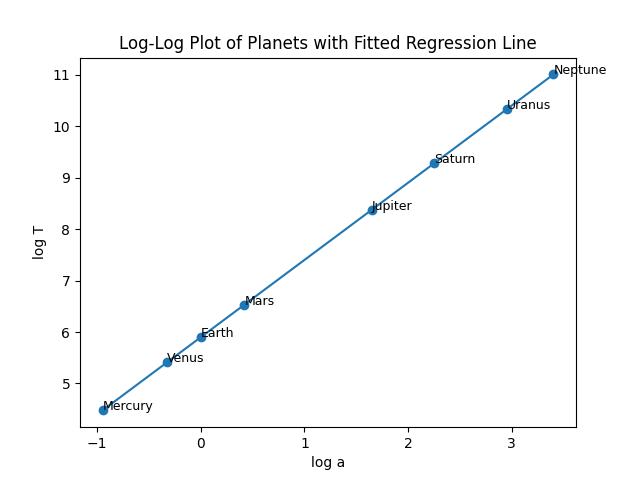
\includegraphics[width=0.8\linewidth]{Figure_1.png}
\caption{Log-log plot of orbital period $T$ versus semi-major axis $a$ for all planets, with fitted regression line.}
\end{figure}


\newpage


\section*{Projection Matrix}
Consider linear regression problem:
\begin{equation}
	\min\limits_{\vx}\frac{1}{2}\|\mA\vx-\vy\|^2_2
\end{equation}
we say the optimal solution is $\vx^*=(\mA^T\mA)^{-1}\mA^T\vy$, which states that any $\vy$ projected to space $\mA$ is given by $\hat{\vy}=\mA\vx^*=\mA(\mA^T\mA)^{-1}\mA^T\vy$, and we define $\mA(\mA^T\mA)^{-1}\mA^T$ as the \textit{projection matrix} $\mathcal{P}$. Please prove that:
\begin{itemize}
%	\item Please verify $\mathcal{P}$ is symmetric
%	\item Show that if each column of $\mA$ is linearly independent, then $\mA^T\mA$ is positive definite and thus invertible
	\item $\mathcal{P}^n=\mathcal{P}$ for any $n$ which is positive integer
	\item Eigenvalue of $\mathcal{P}$ is either $0$ or $1$
	\item $trace(\mathcal{P})=rank(\mathcal{P})$
\end{itemize}
After you have proved all the above, please use Python/Matlab to randomly generate $\mA$ (more rows than columns, say $\mA\in\R^{10\times5}$) and manually verify the correctness of the above conclusions.
%Why might we prefer to minimize the sum of absolute residuals instead of the residual sum of squares for some data sets? Recall clustering method $K$-means when calculating the controid, it is to take the mean value of the datapoints belonging to the same cluster, so what about $K$-medians? What is its advantage over of $K$-means? Please use a synthetic (toy) experiment to illustrate your conclusion.
% \vspace{4cm}
%\section*{Problem 5}
% Please show that:
% \begin{enumerate}
% 	\item if a matrix is symmetric, denote its eigenvalue and singular value as $\bm{\lambda}, \bm{\sigma}$ respectively (descending order in magnitude), then we have: $\bm{\lambda}^2=\bm{\sigma}^2$.
% 	\item if the matrix is symmetric and positive definite, then $\bm{\lambda}=\bm{\sigma}$.
% 	\item for PCA, the loading vectors can be directly computed from the $q$ columns of  $\mU$ where  $[\mU,\mS,\mU]=svd(\mX^T\mX)$, please show that any $[\pm\vu_1,\pm\vu_2,\dots,\pm\vu_q]$ will be equivalent to $[\vu_1,\vu_2,\dots,\vu_q]$ in terms of the same variance while satisying the orthonormality constraint.
% \end{enumerate}  

Consider the least-squares problem
\[
\min_{\vx}\frac12\|\mA\vx-\vy\|_2^2,
\]
where $\mA\in\mathbb{R}^{m\times n}$ (assume $\mA$ has full column rank so that $\mA^T\mA$ is invertible).
The optimal solution is
\[
\vx^*=(\mA^T\mA)^{-1}\mA^T\vy.
\]
The projection of $\vy$ onto $\mathrm{col}(\mA)$ is
\[
\hat{\vy}=\mA\vx^*=\mA(\mA^T\mA)^{-1}\mA^T\vy.
\]
Define the projection matrix
\[
\mathcal{P} := \mA(\mA^T\mA)^{-1}\mA^T.
\]

\subsection*{1) Prove $\mathcal{P}^n=\mathcal{P}$ for any positive integer $n$ (Induction)}

Recall
\[
\mathcal{P}=\mA(\mA^T\mA)^{-1}\mA^T.
\]
First compute $\mathcal{P}^2$:
\begin{align*}
\mathcal{P}^2
&=\Big(\mA(\mA^T\mA)^{-1}\mA^T\Big)\Big(\mA(\mA^T\mA)^{-1}\mA^T\Big)\\
&=\mA(\mA^T\mA)^{-1}(\mA^T\mA)(\mA^T\mA)^{-1}\mA^T\\
&=\mA(\mA^T\mA)^{-1}\mA^T\\
&=\mathcal{P}.
\end{align*}

We now prove by induction that $\mathcal{P}^n=\mathcal{P}$ for all integers $n\ge 1$.

\textbf{Base case ($n=1$):}
\[
\mathcal{P}^1=\mathcal{P},
\]
which is true.

\textbf{Inductive hypothesis:} Assume for some $k\ge 1$ that
\[
\mathcal{P}^k=\mathcal{P}.
\]

\textbf{Inductive step:} Then
\[
\mathcal{P}^{k+1}=\mathcal{P}^k\mathcal{P}.
\]
Using the inductive hypothesis $\mathcal{P}^k=\mathcal{P}$,
\[
\mathcal{P}^{k+1}=\mathcal{P}\mathcal{P}=\mathcal{P}^2.
\]
From the earlier computation $\mathcal{P}^2=\mathcal{P}$, we obtain
\[
\mathcal{P}^{k+1}=\mathcal{P}.
\]

Therefore, by mathematical induction, $\mathcal{P}^n=\mathcal{P}$ for all integers $n\ge 1$.

\subsection*{2) Eigenvalues of $\mathcal{P}$ are either $0$ or $1$}

Let $\vlambda$ be an eigenvalue of $\mathcal P$ with eigenvector $\vv$:
\[
\mathcal P\vv=\lambda\vv.
\]
Applying $\mathcal P$ again gives
\[
\mathcal P^2\vv=\lambda^2\vv.
\]
Since $\mathcal P^2=\mathcal P$, we also have
\[
\mathcal P^2\vv=\mathcal P\vv=\lambda\vv.
\]
Thus
\[
\lambda^2\vv=\lambda\vv.
\]
Because $\vv\neq0$, this implies
\[
\lambda^2=\lambda,
\]
so
\[
\lambda(\lambda-1)=0.
\]
Hence $\lambda=0$ or $\lambda=1$.

\subsection*{3) Show $\mathrm{trace}(\mathcal{P})=\mathrm{rank}(\mathcal{P})$}

The trace of a matrix equals the sum of its eigenvalues, while the rank equals the number of nonzero eigenvalues.
From part (2), the eigenvalues of $\mathcal P$ are only $0$ or $1$.
Therefore, both $\mathrm{trace}(\mathcal P)$ and $\mathrm{rank}(\mathcal P)$ equal the number of eigenvalues equal to $1$, implying
\[
\mathrm{trace}(\mathcal P)=\mathrm{rank}(\mathcal P).
\]

\subsection*{Numerical verification in Python}

I randomly generated $\mA\in\mathbb{R}^{10\times5}$ and constructed
\[
\mathcal P=\mA(\mA^T\mA)^{-1}\mA^T.
\]

Verified numerically that
\[
\|\mathcal P^n-\mathcal P\|_F\approx 0
\]
for several values of $n$, confirming $\mathcal P^n=\mathcal P$.

The eigenvalues of $\mathcal P$ were approximately
\[
\{1,1,1,1,1,0,0,0,0,0\},
\]
confirming that all eigenvalues are either $0$ or $1$.

Furthermore,
\[
\mathrm{trace}(\mathcal P)=5,\qquad \mathrm{rank}(\mathcal P)=5,
\]
which verifies $\mathrm{trace}(\mathcal P)=\mathrm{rank}(\mathcal P)$.

\begin{lstlisting}
import numpy as np

np.random.seed(0)

m, n = 10, 5
A = np.random.randn(m, n)

# Build projection matrix P = A (A^T A)^{-1} A^T
AtA = A.T @ A
P = A @ np.linalg.inv(AtA) @ A.T

# 1) Verify P^n = P (numerically)
for power in [2, 3, 5, 10]:
    diff = np.linalg.norm(np.linalg.matrix_power(P, power) - P, ord='fro')
    print(f"||P^{power} - P||_F = {diff:.3e}")

# 2) Eigenvalues should be ~ 0 or 1
eigvals = np.linalg.eigvals(P)
eigvals_sorted = np.sort(np.real(eigvals))[::-1]
print("\nEigenvalues (sorted):")
print(np.round(eigvals_sorted, 10))

# Check closeness to 0 or 1
dist_to_0 = np.min(np.abs(eigvals_sorted - 0))
dist_to_1 = np.min(np.abs(eigvals_sorted - 1))
print(f"\nMin distance to 0: {dist_to_0:.3e}")
print(f"Min distance to 1: {dist_to_1:.3e}")

# 3) trace(P) = rank(P)
tr = np.trace(P)
rk = np.linalg.matrix_rank(P)
print(f"\ntrace(P) = {tr:.10f}")
print(f"rank(P)  = {rk}")
\end{lstlisting}

\newpage
\section*{Polynomial Regression}
Assume you have 5 observation samples $\{\{1,1\},\{2,3\},\{3,9\},\{4,15\},\{5,24\}\}$, now please use a Polynomial regression (order 3) model to approximate the samples, please plot the scatter of samples and then plot the function of the regression model. You are expected to output an image similar to the following:
\begin{figure}[h!]
	\centering
	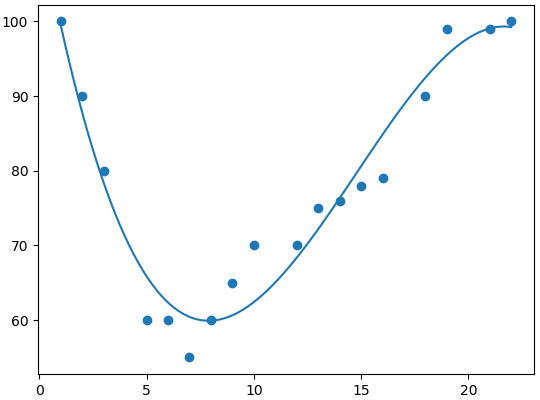
\includegraphics[width=0.5\linewidth]{img_polynomial_regression}
	\caption{Fitting with Polynomial Regression.}
	\label{fig:imgpolynomialregression}
\end{figure}

\subsection*{Python Code}
\begin{lstlisting}
import numpy as np
import matplotlib.pyplot as plt

# Data
x = np.array([1, 2, 3, 4, 5], dtype=float)
y = np.array([1, 3, 9, 15, 24], dtype=float)

# fit cubic polynomial: y = a3 x^3 + a2 x^2 + a1 x + a0
coeffs = np.polyfit(x, y, deg=3)
poly = np.poly1d(coeffs)

print("Cubic coefficients [a3, a2, a1, a0]:")
print(coeffs)

# curve
x_plot = np.linspace(x.min(), x.max(), 400)
y_plot = poly(x_plot)

# plotting
plt.figure()
plt.scatter(x, y)          # sample points
plt.plot(x_plot, y_plot)   # fitted curve

plt.xlabel("x")
plt.ylabel("y")
plt.title("Fitting with Polynomial Regression (Order 3)")
\end{lstlisting}

\begin{figure}[h!]
	\centering
	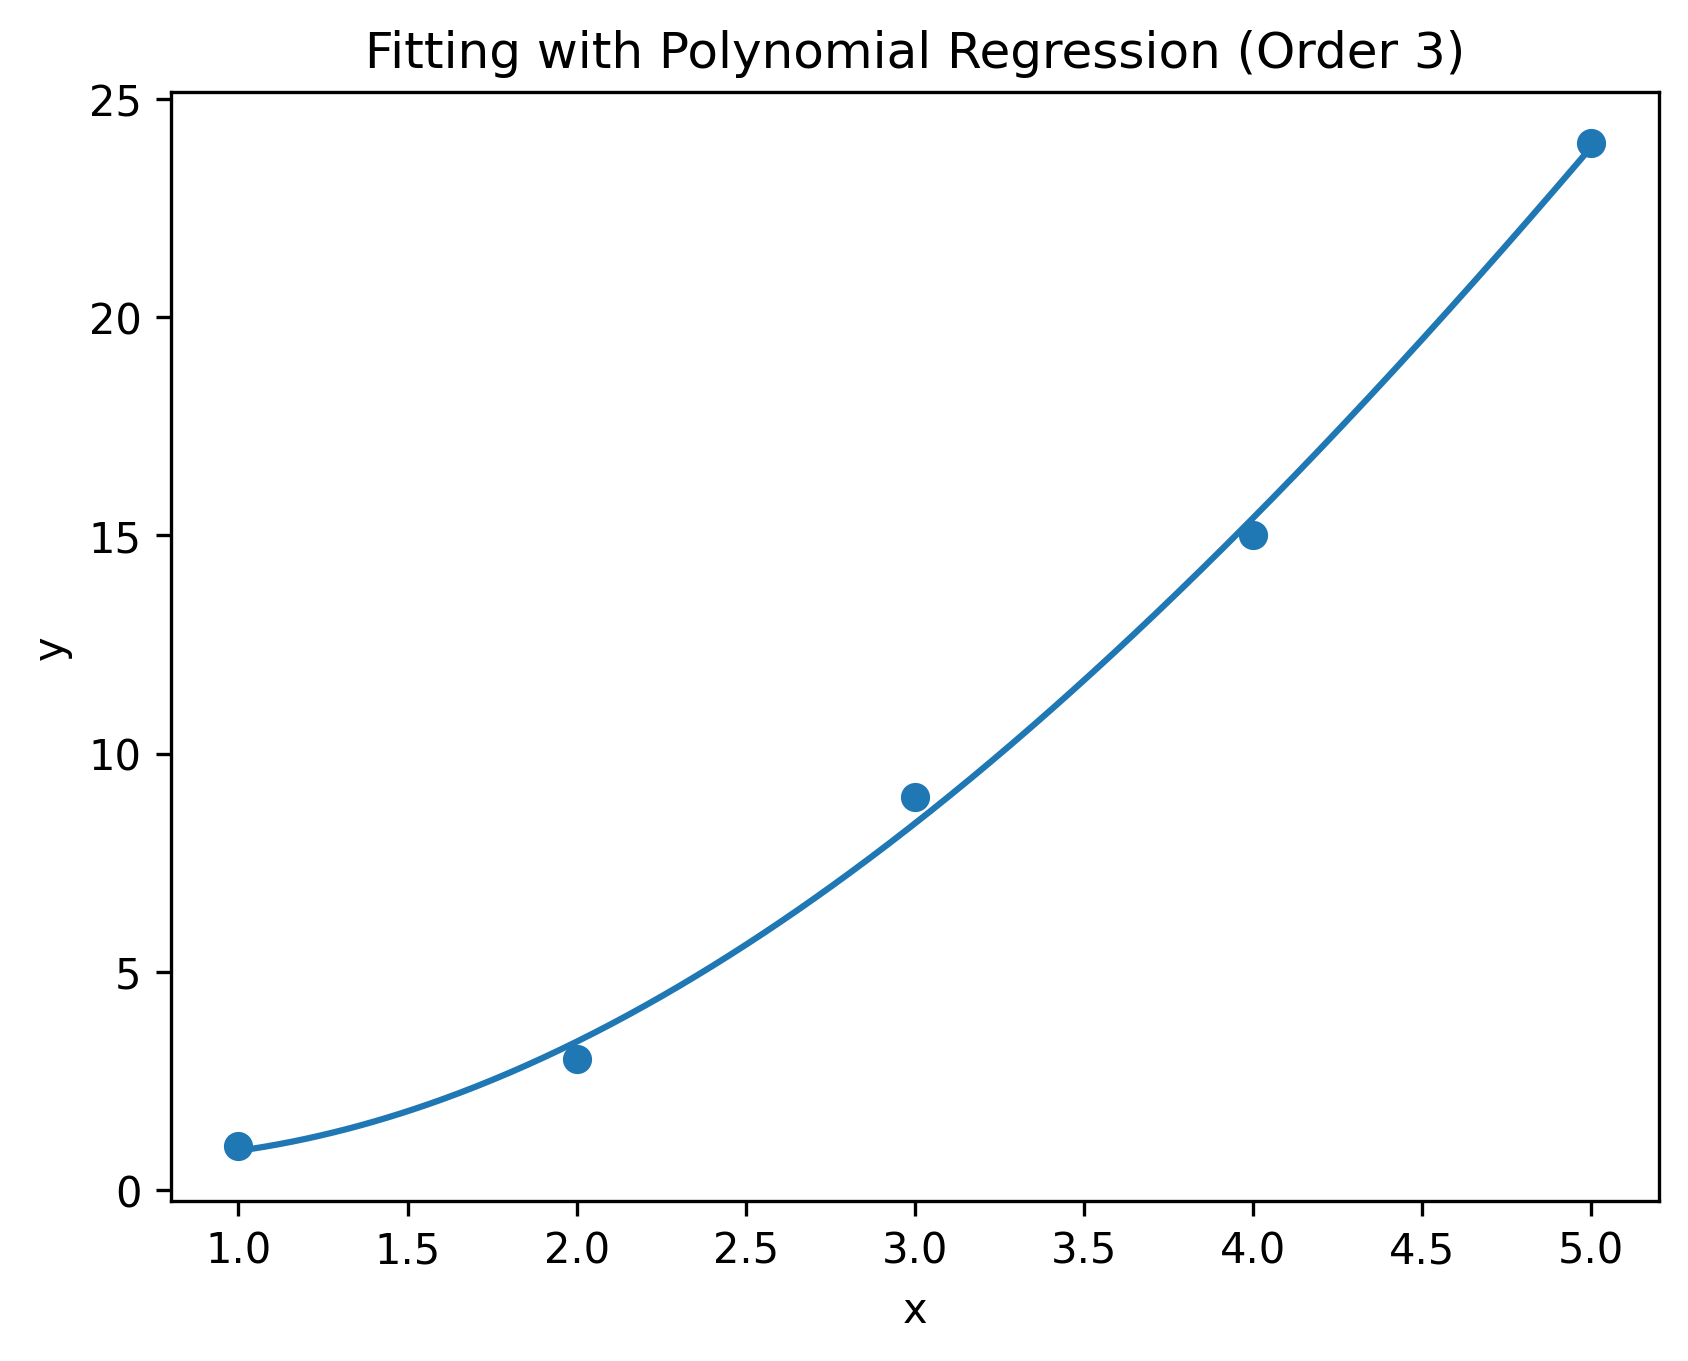
\includegraphics[width=0.55\linewidth]{polyregression.png}
	\caption{Fitting with Polynomial Regression (order 3).}
	\label{fig:polynomialregression}
\end{figure}

 \newpage

 
\section*{Multiple Linear Regression and Variants for Predicting MPG}
 Please find the data \href{https://github.com/selva86/datasets/blob/master/Auto.csv}{here}, now  follow the steps below:
\begin{itemize}
	\item Extract column `cylinders', `displacement', `horsepower', `weight' and `acceleration' as the input features  and column `mpg' as the  response ($\vy$).
	\item Randomly split the data into training and testing subsets (at a ratio of 4:1)
	\item Normalize (via \textit{StandardScaler}) the training samples.
	\item Use a multiple linear regression model to fit the training data.
	\item Make the prediction for testing data and calculate the \textit{Mean Squared Error}. (reminder: you should normalize testing data via the standardscalar earlier)
	\item Fit a \textbf{ridge regression} model on the training data.
	\begin{itemize}
		\item Consider a grid of regularization parameters 
		$\lambda \in \{\lambda_1, \lambda_2, \ldots, \lambda_K\}$.
		\item For each $\lambda$, train the ridge regression model using the normalized training data.
		\item Evaluate the model by computing the Mean Squared Error (MSE) on the testing data.
		\item Report the value of $\lambda$ that yields the lowest testing MSE and the corresponding MSE.
	\end{itemize}
	
	\item Fit a \textbf{lasso regression} model on the training data.
	\begin{itemize}
		\item Use the same grid of regularization parameters $\lambda$ as in the ridge regression.
		\item Train the lasso regression model for each $\lambda$ using the normalized training data.
		\item Evaluate the testing MSE for each $\lambda$.
		\item Identify the best $\lambda$ based on the lowest testing MSE.
		\item Report the selected model coefficients and comment on sparsity.
	\end{itemize}
	
	\item Compare the performance of \textbf{multiple linear regression}, \textbf{ridge regression}, and \textbf{lasso regression}.
	\begin{itemize}
		\item Compare their testing MSEs.
		\item Discuss the effect of regularization on prediction accuracy.
		\item Discuss differences in coefficient magnitudes and feature selection.
	\end{itemize}
	
\end{itemize}

\subsection*{Python Code}
\begin{lstlisting}
import pandas as pd
import numpy as np
from sklearn.model_selection import train_test_split
from sklearn.preprocessing import StandardScaler
from sklearn.linear_model import LinearRegression, Ridge, Lasso
from sklearn.metrics import mean_squared_error

# Load dataset
url = "https://raw.githubusercontent.com/selva86/datasets/master/Auto.csv"
df = pd.read_csv(url)

# Replace missing horsepower values and drop NA
df['horsepower'] = pd.to_numeric(df['horsepower'], errors='coerce')
df = df.dropna()

# Features and target
X = df[['cylinders', 'displacement', 'horsepower', 'weight', 'acceleration']]
y = df['mpg']

# Train-test split (4:1)
X_train, X_test, y_train, y_test = train_test_split(
    X, y, test_size=0.2, random_state=0
)

# Normalize
scaler = StandardScaler()
X_train_scaled = scaler.fit_transform(X_train)
X_test_scaled = scaler.transform(X_test)

# Linear Regression 
lr = LinearRegression()
lr.fit(X_train_scaled, y_train)
y_pred_lr = lr.predict(X_test_scaled)
mse_lr = mean_squared_error(y_test, y_pred_lr)

print("Linear Regression MSE:", mse_lr)

# Lambda grid
lambdas = np.logspace(-3, 3, 20)

# Ridge Regression
ridge_mses = []
for l in lambdas:
    ridge = Ridge(alpha=l)
    ridge.fit(X_train_scaled, y_train)
    pred = ridge.predict(X_test_scaled)
    ridge_mses.append(mean_squared_error(y_test, pred))

best_ridge_lambda = lambdas[np.argmin(ridge_mses)]
best_ridge_mse = min(ridge_mses)

print("\nBest Ridge Lambda:", best_ridge_lambda)
print("Best Ridge MSE:", best_ridge_mse)

# Lasso Regression 
lasso_mses = []
lasso_models = []

for l in lambdas:
    lasso = Lasso(alpha=l, max_iter=10000)
    lasso.fit(X_train_scaled, y_train)
    pred = lasso.predict(X_test_scaled)
    lasso_mses.append(mean_squared_error(y_test, pred))
    lasso_models.append(lasso)

best_lasso_idx = np.argmin(lasso_mses)
best_lasso_lambda = lambdas[best_lasso_idx]
best_lasso_mse = lasso_mses[best_lasso_idx]
best_lasso_model = lasso_models[best_lasso_idx]

print("\nBest Lasso Lambda:", best_lasso_lambda)
print("Best Lasso MSE:", best_lasso_mse)

print("\nLasso Coefficients:")
for name, coef in zip(X.columns, best_lasso_model.coef_):
    print(f"{name}: {coef:.4f}")
\end{lstlisting}

\subsection*{Results and Comparison}

The testing Mean Squared Error (MSE) for multiple linear regression was
\[
\text{MSE}_{\text{linear}} = 19.0035.
\]

\paragraph{Ridge Regression}
Using a logarithmically spaced grid of $\lambda\in[10^{-3},10^{3}]$, the optimal ridge parameter was
\[
\lambda_{\text{ridge}} = 26.37,
\]
with corresponding testing MSE
\[
\text{MSE}_{\text{ridge}} = 18.2933.
\]

\paragraph{Lasso Regression}
Using the same grid, the best lasso parameter was
\[
\lambda_{\text{lasso}} = 0.336,
\]
with testing MSE
\[
\text{MSE}_{\text{lasso}} = 18.5590.
\]

The lasso model selected the following coefficients:
\[
\text{cylinders}=-0.3626,\quad
\text{horsepower}=-1.3960,\quad
\text{weight}=-4.6288,
\]
while \textit{displacement} and \textit{acceleration} were shrunk to zero.

\paragraph{Discussion}
Ridge regression achieved the lowest testing MSE, indicating improved generalization compared to standard linear regression.
Lasso regression produced a sparse model by eliminating displacement and acceleration, demonstrating automatic feature selection.
Regularization reduces coefficient magnitudes and mitigates multicollinearity among correlated predictors such as displacement, horsepower, and weight.
Overall, ridge provided the best predictive performance, while lasso offered interpretability through sparsity.


\end{document}
